Para pilares com seções mais complexas, deve-se obter um pilar retangular equivalente, de modo que se possa utilizar os métodos já vistos.

\begin{figure}[H]
	\begin{center}
	\caption{Vista em planta de um pilar com seção "L".}
    	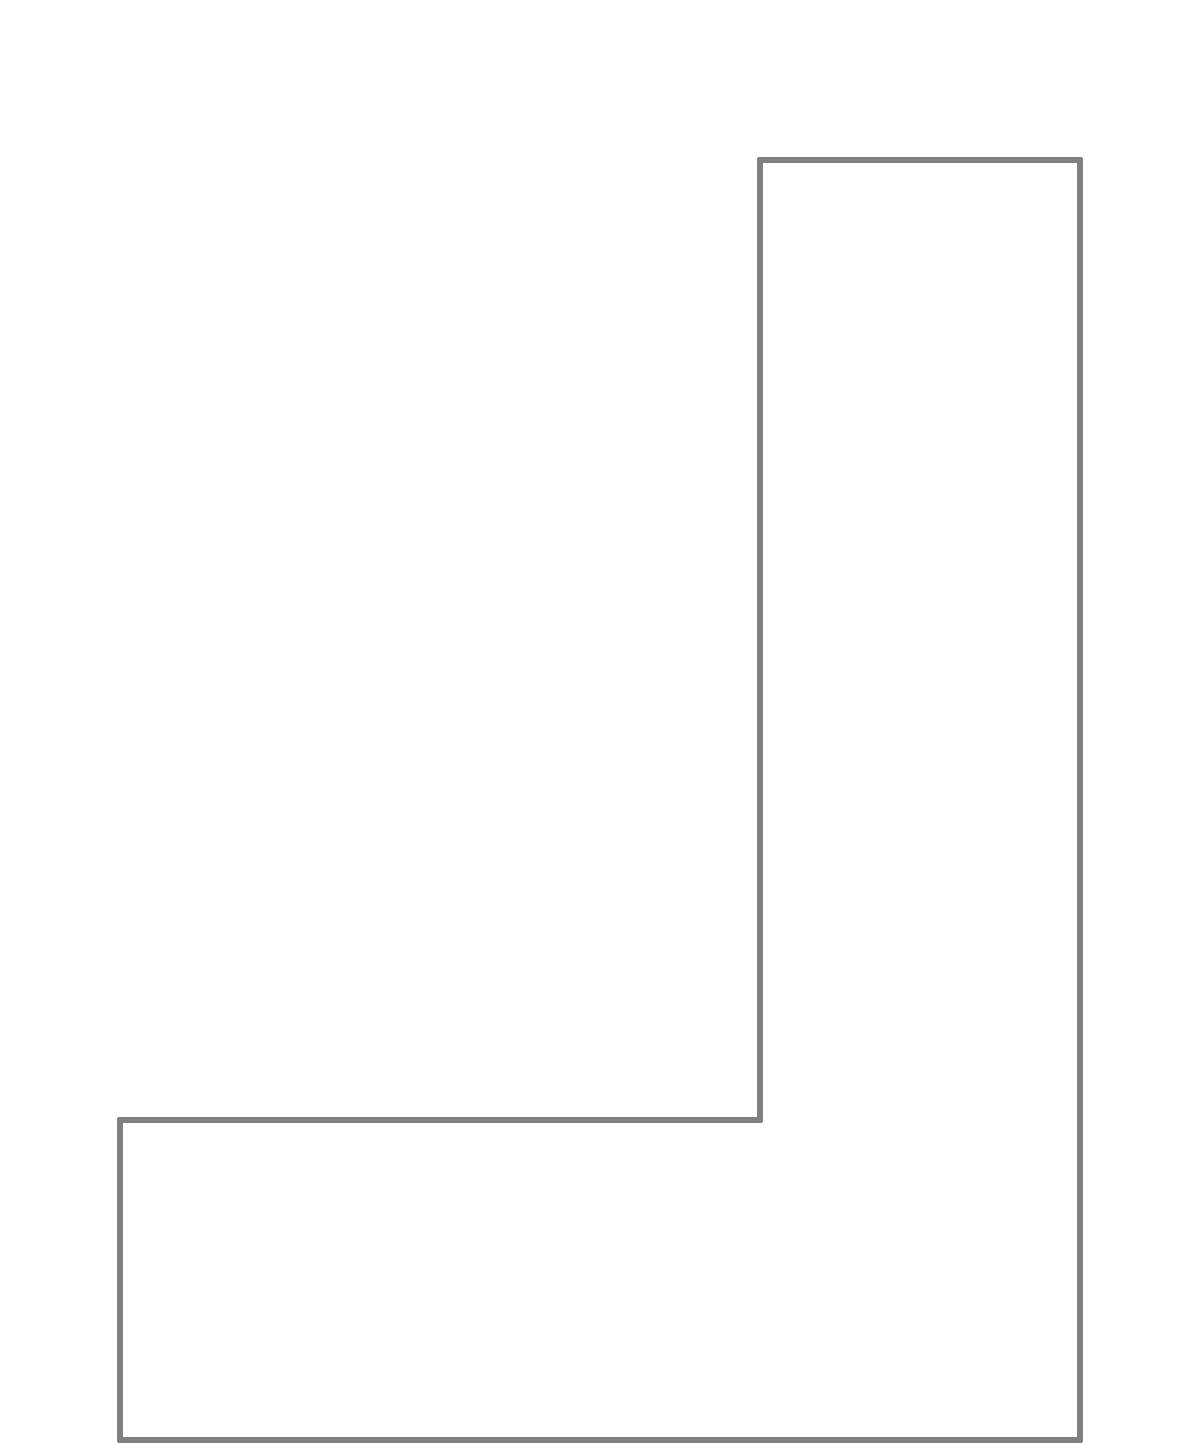
\includegraphics[width=0.25\textwidth]{Fundacoes-rasas-ou-diretas/Imagens/Sapatas-com-secao-LUZ.png}
	\end{center}
\end{figure}

O primeiro passo é subdividir a figura inicial em figuras menores de geometria conhecida (preferencialmente retangular), cada qual com seu respectivo centro geométrico (CG), como segue:

\begin{figure}[H]
	\begin{center}
	\caption{Vista em planta da subdivisão do pilar em "L" em geometrias mais simples.}
    	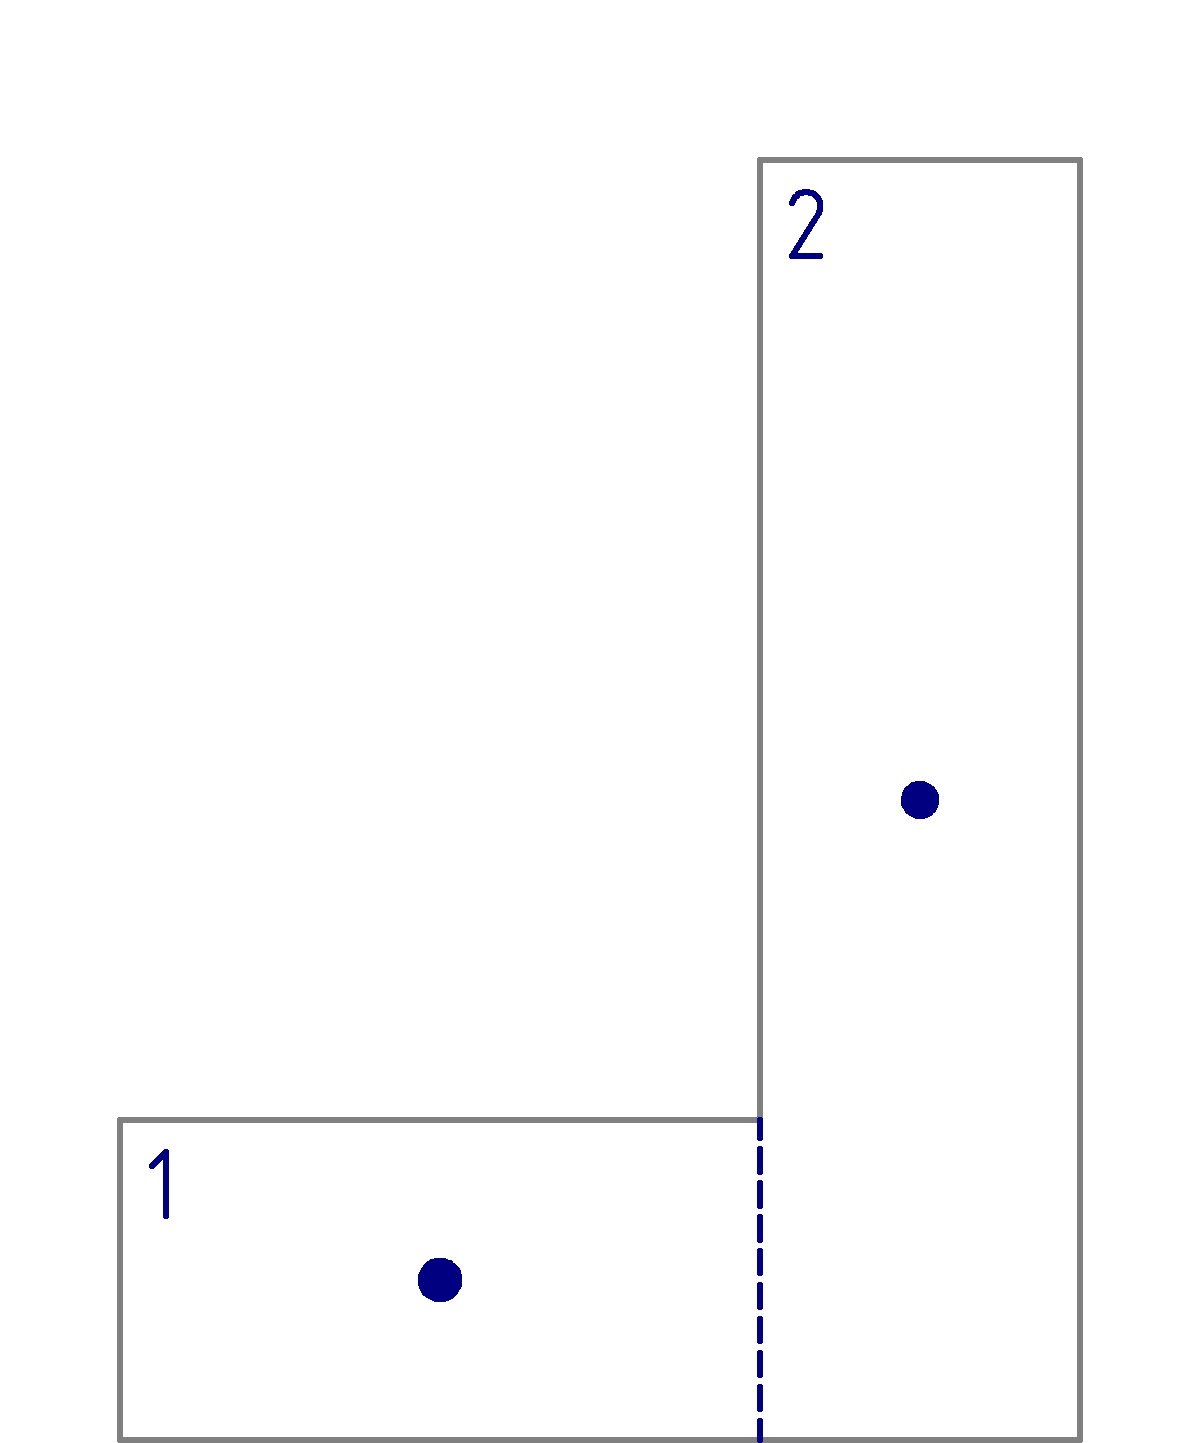
\includegraphics[width=0.25\textwidth]{Fundacoes-rasas-ou-diretas/Imagens/Sapatas-com-secao-LUZ-2.png}
	\end{center}
\end{figure}

Essa subdivisão permite o cálculo das coordenadas do CG da figura mais complexa pelas seguintes médias ponderadas:

\begin{equation}x_{CG}=\frac{\displaystyle\sum_{i=1}^{n} A_i\cdot \overline{x}_i}{\displaystyle\sum_{i=1}^{n} A_i}\end{equation}
\begin{equation}y_{CG}=\frac{\displaystyle\sum_{i=1}^{n} A_i\cdot \overline{y}_i}{\displaystyle\sum_{i=1}^{n} A_i}\end{equation}

Onde $x_{CG}$ e $y_{CG}$ são as coordenadas do CG da figura final; $A_i$ é a área da figura $i$; e $\overline{x}_i$ ou $\overline{y}_i$ é a coordenada do CG da figura fracionada $i$.

Além disso, antes de calcular os pontos de CG da figura mais complexa, coloca-se eixos de referência na figura, como segue:

\begin{figure}[H]
	\begin{center}
	\caption{Vista em planta da colocação de eixos para encontrar o CG.}
    	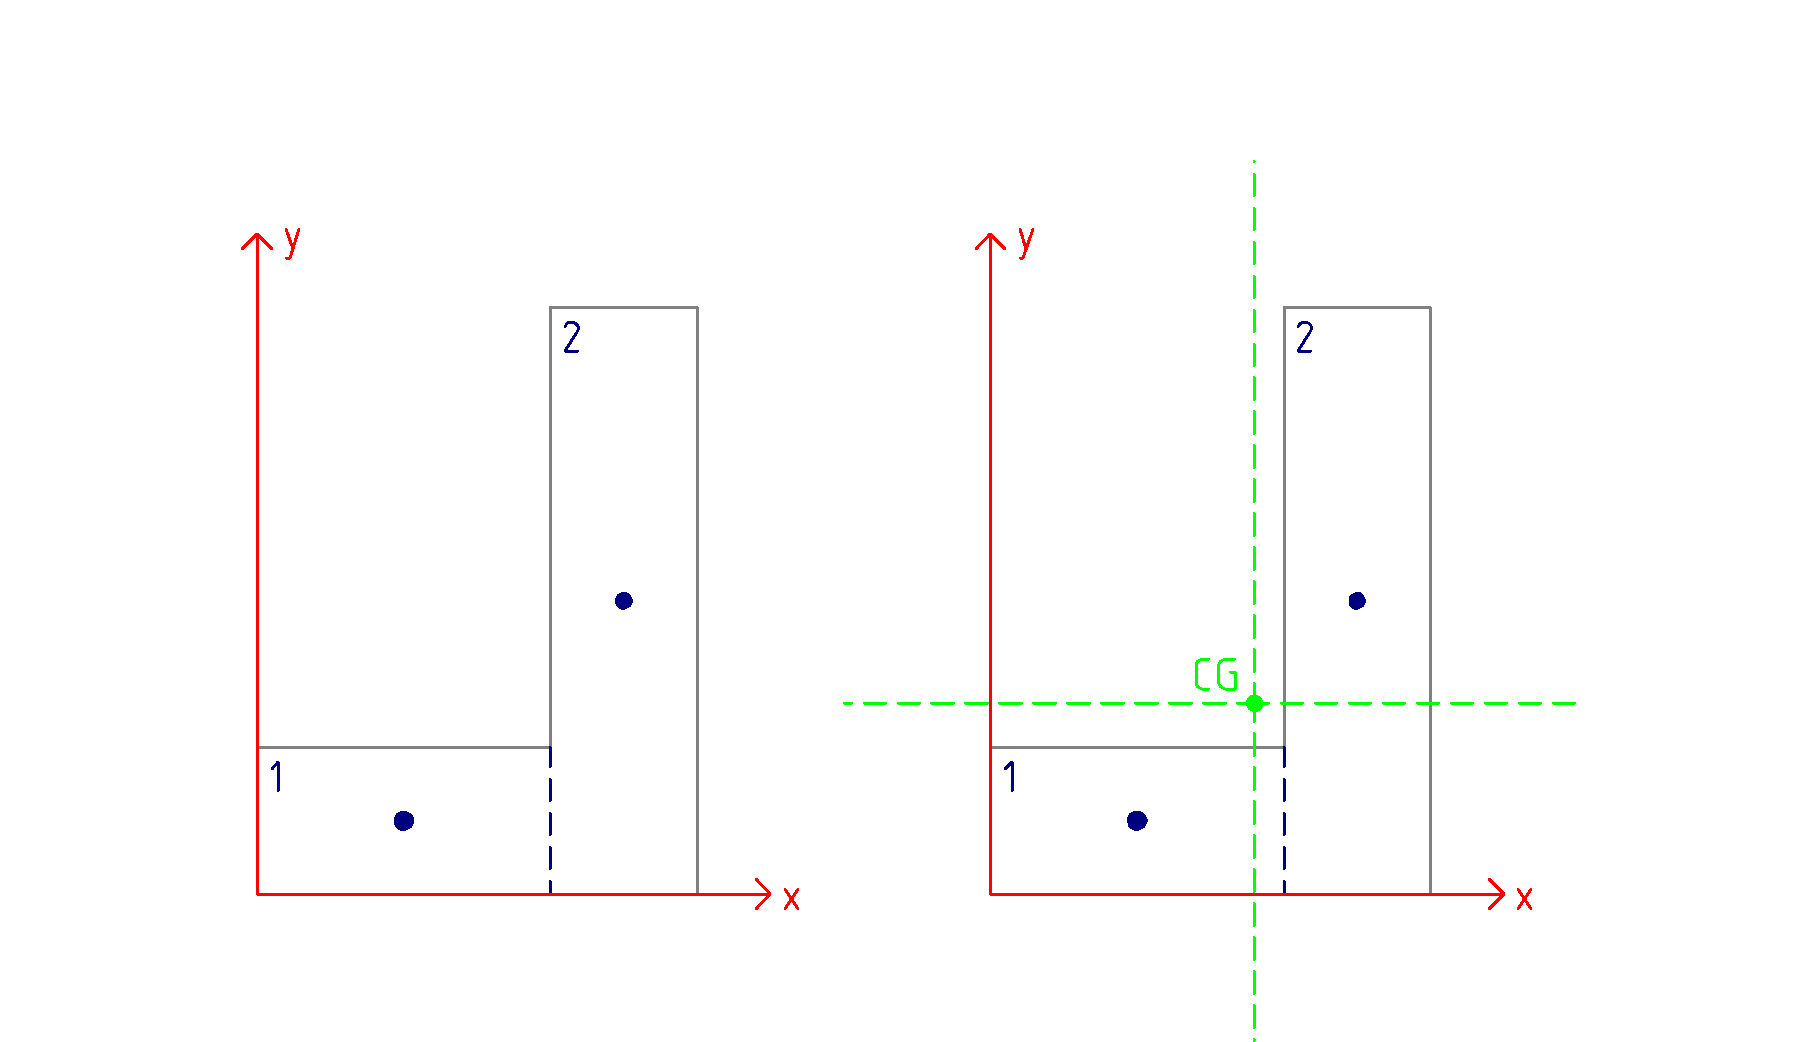
\includegraphics[width=0.85\textwidth]{Fundacoes-rasas-ou-diretas/Imagens/Sapatas-com-secao-LUZ-3.png}
	\end{center}
\end{figure}

Agora, deve-se checar, a partir dos eixos traçados, qual a maior distância de ambas as superfícies da peça em cada eixo até o ponto CG, ou seja:

\begin{figure}[H]
	\begin{center}
	\caption{Vista em planta da checagem da distância de cada extremidade em relação ao CG da figura principal.}
    	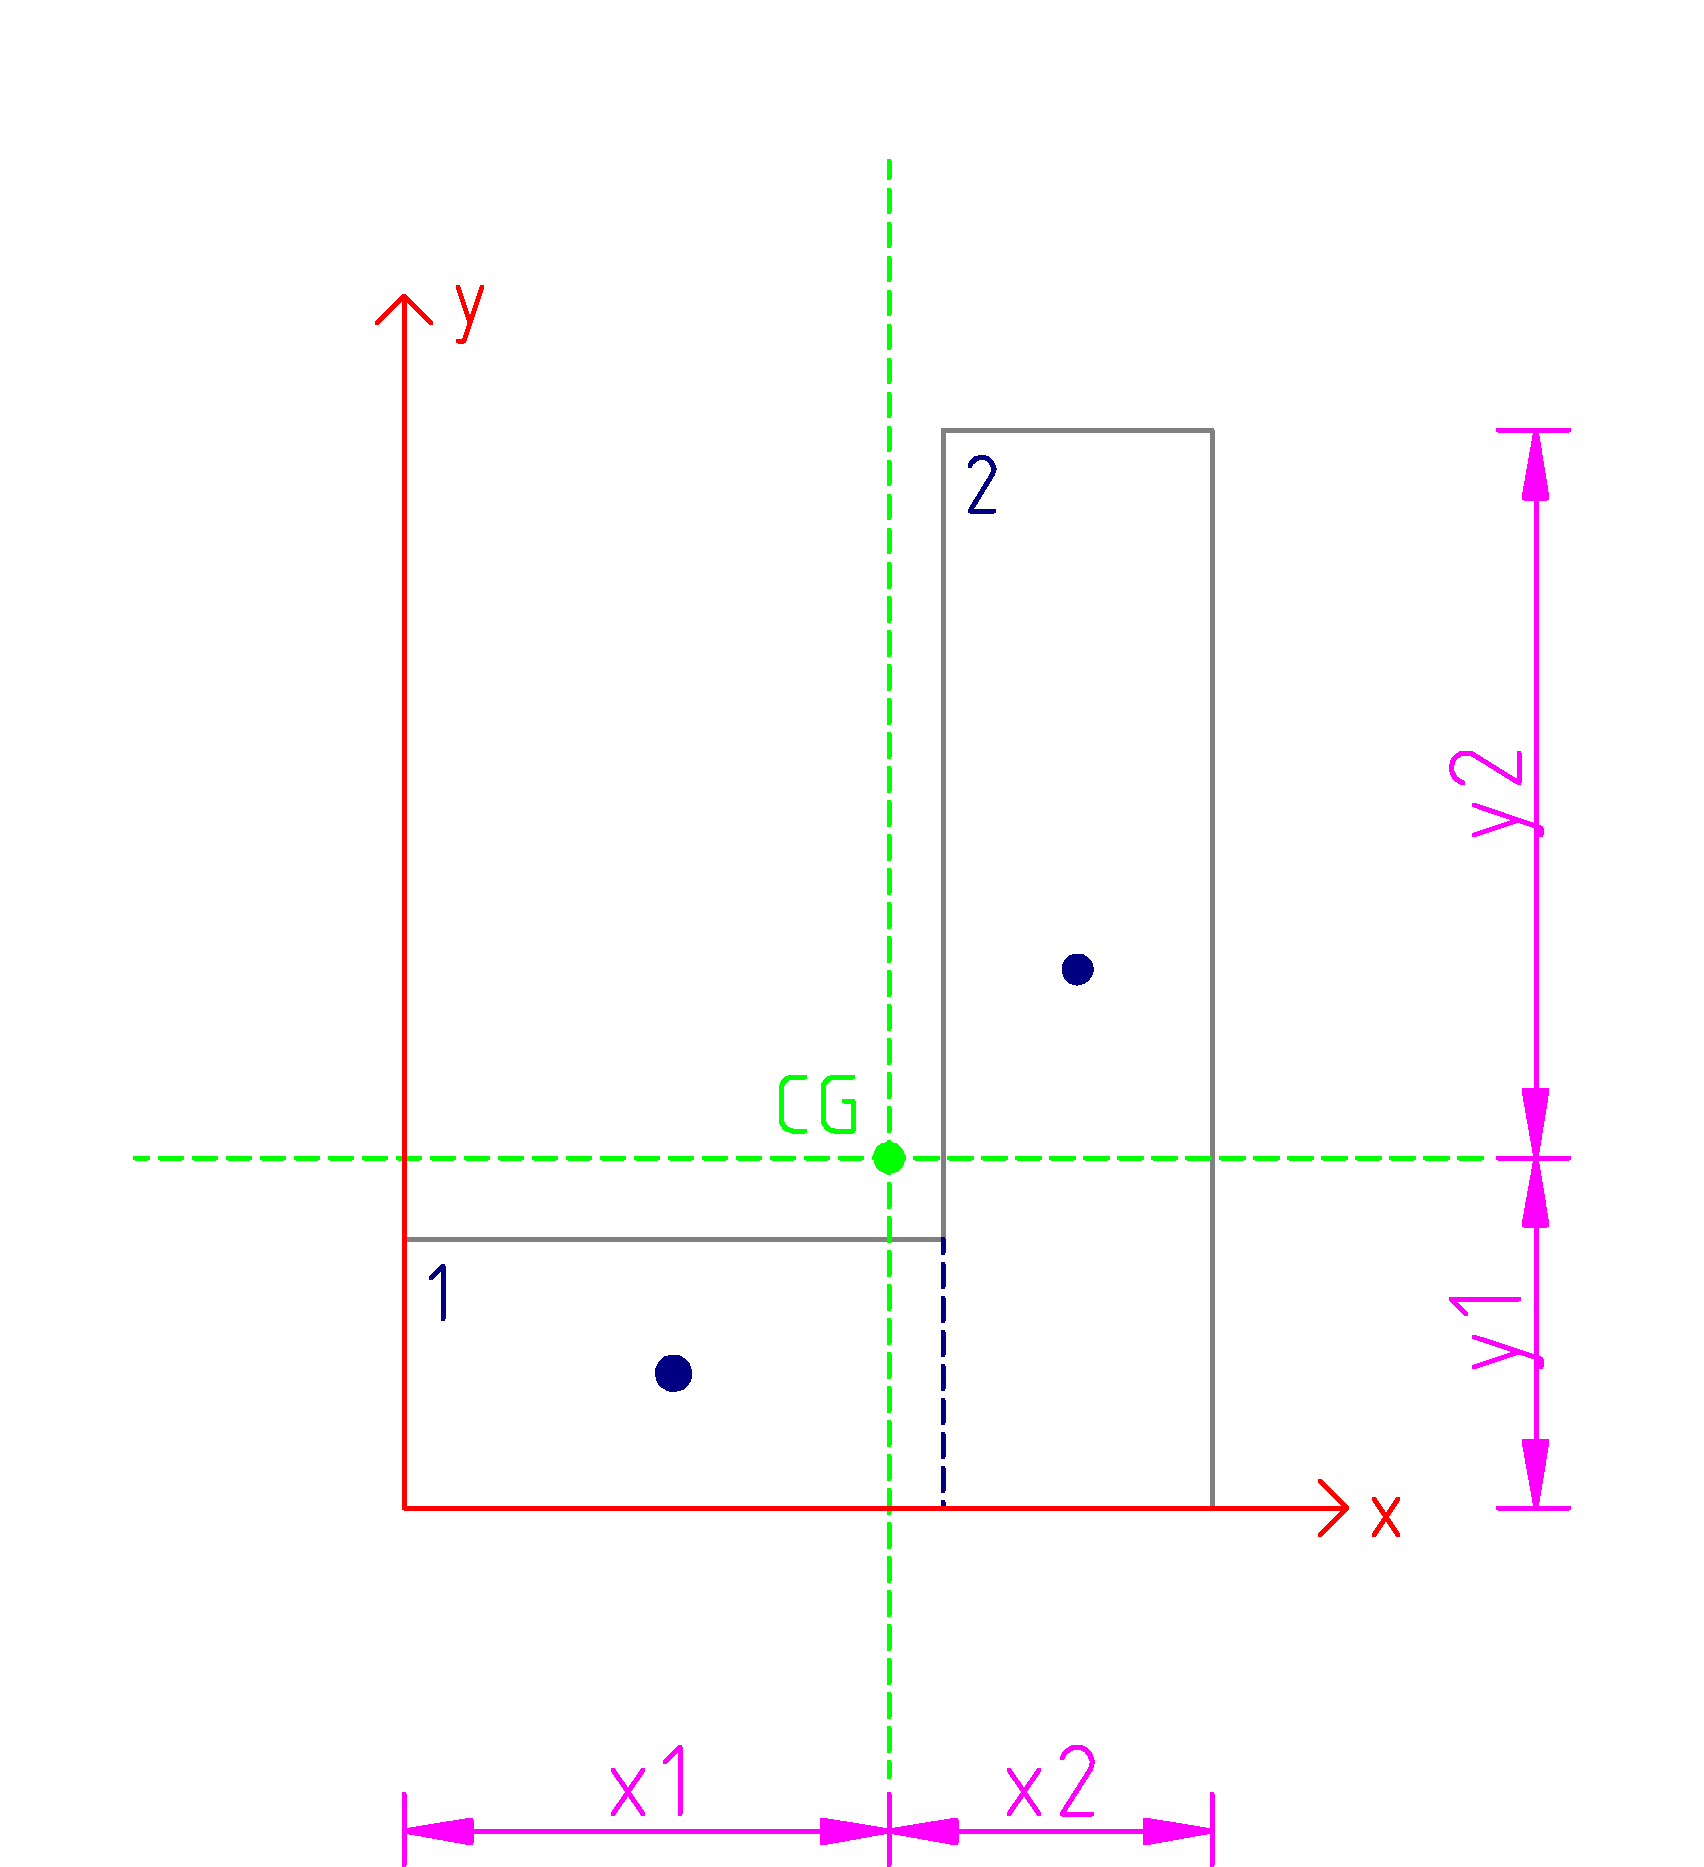
\includegraphics[width=0.45\textwidth]{Fundacoes-rasas-ou-diretas/Imagens/Sapatas-com-secao-LUZ-4.png}
	\end{center}
\end{figure}

O maior valor deve ser dobrado para cada eixo. Assim, o pilar retangular equivalente com mesmo CG é obtido.

\begin{figure}[H]
	\begin{center}
	\caption{Vista em planta dos comprimentos do pilar retangular equivalente para a seção em "L".}
    	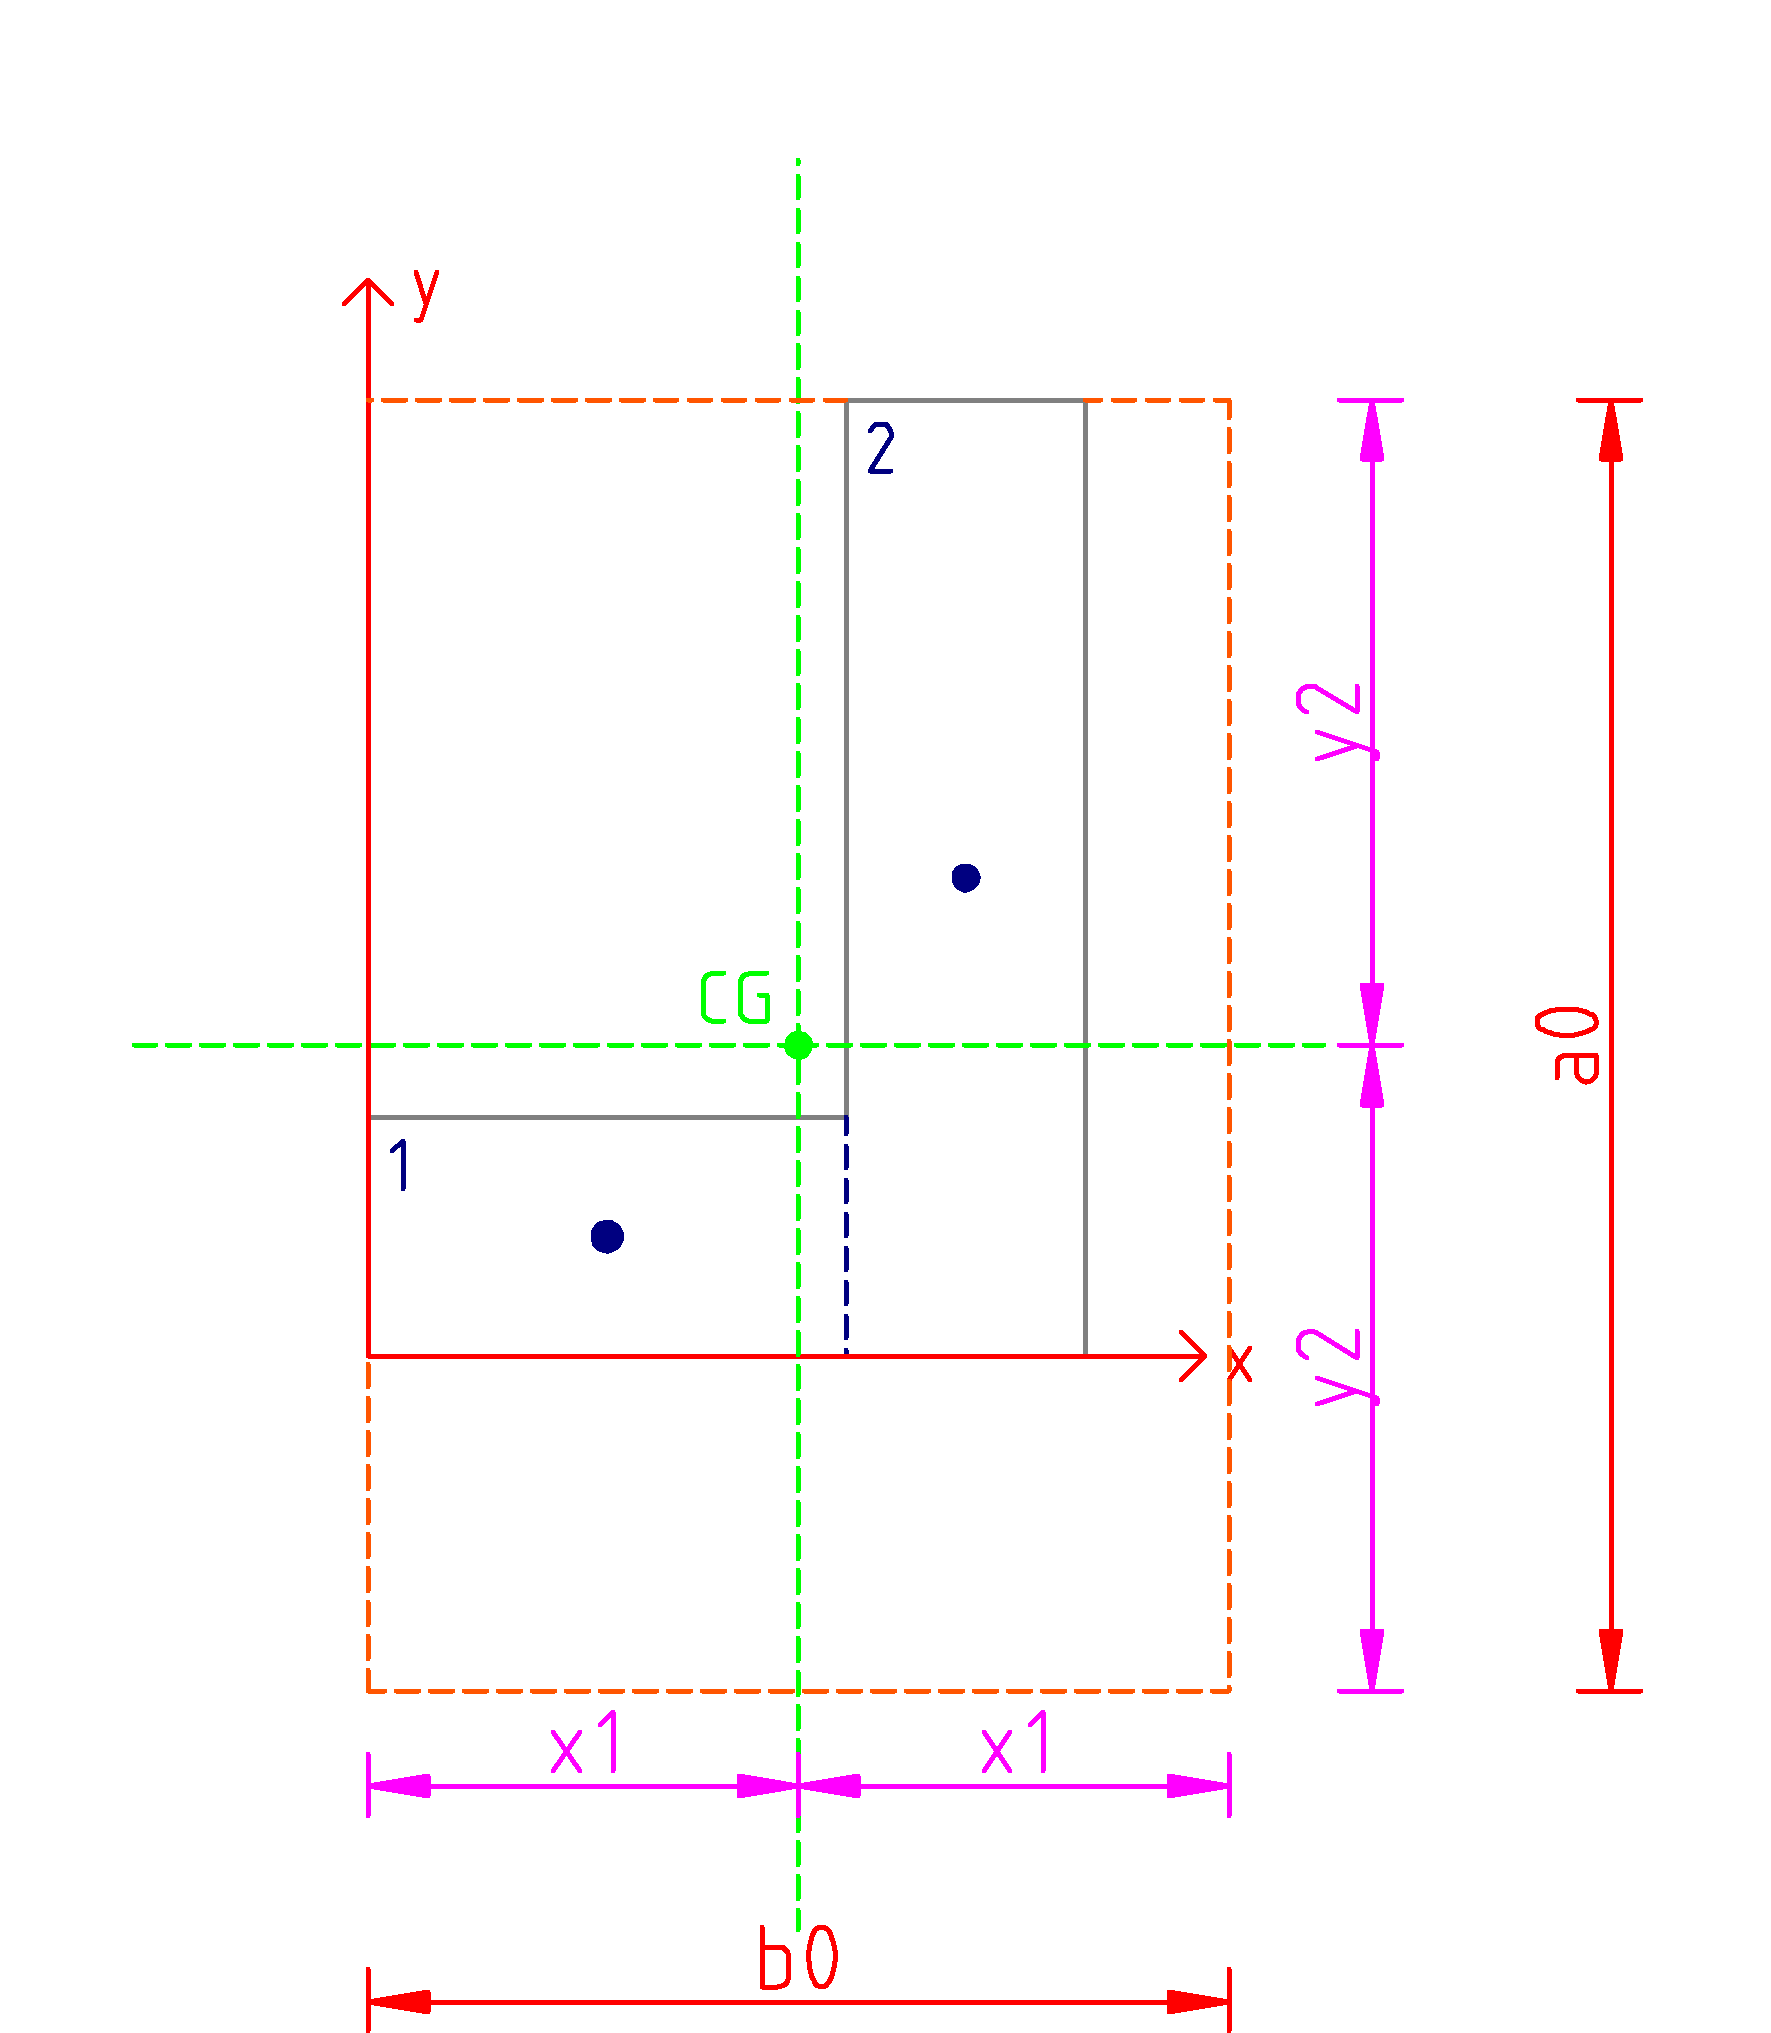
\includegraphics[width=0.45\textwidth]{Fundacoes-rasas-ou-diretas/Imagens/Sapatas-com-secao-LUZ-5.png}
	\end{center}
\end{figure}